\documentclass[lettersize,journal]{IEEEtran}
\usepackage{amsmath,amsfonts}
\usepackage{algorithmic}
\usepackage{algorithm}
\usepackage{array}
\usepackage[caption=false,font=normalsize,labelfont=sf,textfont=sf]{subfig}
\usepackage{textcomp}
\usepackage{stfloats}
\usepackage{url}
\usepackage{verbatim}
\usepackage{graphicx}
\usepackage{cite}
\usepackage[hypcap=false]{caption}
\usepackage{float}

% Set path for images
\graphicspath{ {./images/} }

\newenvironment{Figure}
    {\par\medskip\noindent\minipage{\linewidth}}
    {\endminipage\par\medskip}


\begin{document}

\title{An Explainable Machine Learning Approach to Antenna Design}

\author{Tyler Carr \\ carrt12@my.erau.edu \\ Embry-Riddle Aeronautical University \\ Daytona Beach, FL}

\maketitle

\begin{abstract}
Antenna design processes require extensive EM (electromagnetic) simulation tasks that are resource and time intensive, which are prone to interruptions. Design equations are only available for a predefined and limited set of antenna geometries. By applying a machine learning algorithm to data that has already been generated from simulations of an antenna, performance metrics can be predicted significantly quicker than running full simulations. Insights about which geometric parameter had the most significant impact on the prediction can be drawn from the model and included in the output. Additionally, the model can be reversed so that for a particular form of antenna, an optimal geometry can be produced that will result in a specified performance and frequency range. 
\end{abstract}

\section{Introduction}
Antenna designs require simulation in order to determine the performance of the antenna. The high-frequency structure simulator (HFSS) is an electromagnetic simulation software which is used to design and simulate antennas between a range of frequencies. When designing the antenna, details such as dimensions of the antenna geometry, materials used for the antenna, and frequency are specified~\cite{Maxworth_2022}. Simulations are then run. These simulations produce $S_{11}$ values, which are the reflection coefficients. These represent the amount of power that is reflected from the antenna, and is measured in decibels. This value is always negative, and a lower value means the antenna is performing more efficiently. Ideally, this value is below -10dB~\cite{Bevelacqua_2015}.


\subsection{Dataset}
Two datasets were used to train and test the machine learning models. Both datasets were generated from a parametric sweep of the antenna. The two antennas that were used were a patch antenna, which can be pictured in~\ref{patch_antenna}, and a leaky wave antenna. The seven features of the patch antenna dataset contained inset\_dist, L, sub\_thick, W, W0, y0, and Freq, with all measurements being in millimeters except frequency being GHz. The seven features of the leaky wave antenna dataset include Feed\_Gap (mm), Feed\_Inset (cm), Feed\_W (cm), Ground\_gap (mm), Pad\_L (cm), Pad\_W (cm), and Freq (GHz). All of the features except the frequency represent a part of the antenna's geometry. Each of the features were paired with a label, which is a $S_{11}$ value.

\subsection{Simulation Issues}
The main issue with running simulations in HFSS is the amount of time that it takes. The matrix operations that are required to run many iterations of simulations to analyze loss can take multiple days to complete~\cite{john_antenna_2009,liu_efficient_2014}. Depending on how the simulation is set up, this process could be impacted by power outages or software bugs, resulting in a loss of data and requiring manual intervention to re-run the simulation. 

HFSS works by specifying a range of dimensions and outputting performance metrics, such as $S_{11}$ values. This is insightful, but there is a degree of trial and error involved in finding an optimal antenna geometry. One would start by specifying what they would think would be the ideal antenna geometry using their own intuition. Based on the results from an initial simulation run, geometry values would be adjusted in an attempt to optimize the geometry.

By using a machine learning algorithm to do the bulk of the investigative work, the amount of simulation iterations that need to be run to optimize an antenna's geometry can be significantly reduced. By training the model on the 405 geometries, frequencies, and $S_{11}$ values, permutations of more geometries and frequencies can be generated computationally and new $S_{11}$ values can be predicted using the model. These predictions can be searched, making it easier and quicker to narrow down to a specific area of interest without having to wait for simulations to run.


\subsection{Reversing the Problem}
After training a machine learning model on the dataset, a table is produced with significantly more rows than was started with from the simulated data. Predictions can be searched by specifying the desired $S_{11}$ value and a range of frequency values that the antenna should operate between. Antenna geometries that match the search are returned, which saves significant time that would be required to set up and perform additional simulations. When seeking an optimal geometry between a certain frequency range, the geometry that results in the $S_{11}$ with the lowest maximum $S_{11}$ range would be chosen.

\section{Related Work}
Machine learning topics with antenna design optimizations have been explored before. The algorithm and methods that are chosen ultimately depend on the way that the antenna geometry is expressed. One format that the input data can have is to be in tabular format, where rows represent combinations of geometry measurements and some performance specification, such as $S_{11}$.

Liu et al.~used three different types of antennas of varying complexity, including antennas with 10, 19, and 7 geometric parameters. They use a Gaussian Process surrogate model and an evolutionary search mechanism~\cite{liu_efficient_2014}. He et al.~combined an ANN with a simulated annealing algorithm of a wideband patch antenna with four geometric parameters~\cite{10318051}. Cui et al.~input a mesh of data into a KNN (K-nearest neighbor) algorithm to optimize parameters quickly with only a limited number of data samples, using only 10\% as many data samples as ANN~\cite{9119820}. Ranjan et al.~compared the performance of five different machine learning algorithms using both $R^2$ score and the mean squared error metric on a coplanar waveguide fed band-notched monopole antenna. These algorithms include Decision Tree, Random Forest, XGBoost, KNN, and ANN.~\cite{ranjan_ultra-wideband_2022}. All of the above examples have decreased both the amount of time taken and the computational expensiveness when compared to typical EM simulations.

There has been less research performed with the intention of reversing the problem and receiving optimized geometry parameters from specified desired antenna performance values. Xiao et al.~applied an inverse ELM (extreme learning machine) and an ANN in an attempt to solve this problem, using multiple different performance metrics instead of just one as the input. The ELM strategy applies two algorithms for classifying similar curves and training~\cite{9063448}. The ANN improves the accuracy of the ELM and helps organize the environment~\cite{XiaoLi-Ye2021IANN}.

\begin{Figure}
\centering
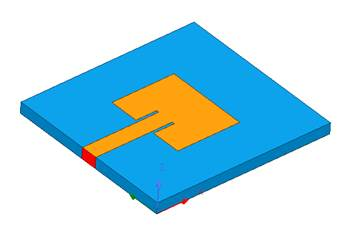
\includegraphics[width=3.0in]{patch_antenna.jpg}
\captionof{figure}{Screenshot of the Patch Antenna}
\label{patch_antenna}
\end{Figure}


\section{Methodology}
In order to determine the optimal antenna geometry, a machine learning algorithm was employed. This algorithm is trained with a supervised learning method using the parametric sweep dataset for the antenna geometry. Because the data is generated from a parametric sweep, it contains many different combinations of geometries. For the patch antenna, out of the 40,905 rows, there were 405 unique geometries that each had a simulated $S_{11}$ value for the same frequency range between 4 to 12.

Generating more data for each geometry feature was done by inserting new values between the minimum and maximum of each feature. Permutations of the geometries and frequencies added up to a total of 9,720 unique geometries, which includes the original 405. The real $S_{11}$ values are used for the original 405, but predictions are generated for the rest of the geometry and frequency combinations. This new dataset includes a total of 981,720 rows. Similarly, for the leaky wave antenna, there were 21 unique geometries that were used as training data between a frequency range between 2 to 20. There were 555 unique geometries in the end for this antenna design. These generated values for each antenna aided in providing a better guess of an optimal geometry for a specfiied $S_{11}$ and frequency range, helping optimize the antenna faster. 

\subsection{Analyzing the Data}
A regression algorithm was chosen as the label is numeric. 20\% of the dataset provided by the parametric sweep was reserved for testing and comparing the performance of the models, and the remaining 80\% was used to train the models.

In order to determine if a $S_{11}$ value was predicted accurately or not, a tolerance was utilized. An exact prediction of an $S_{11}$ value with high precision is very unlikely, so this tolerance allows for some flexibility. The tolerance is the error that we allow the value to contain, and we consider the prediction accurate if it is within the range specified by the tolerance either above or below the true value. This concept is used when calculating the score of a model~\eqref{eq:tolerance}, with $\epsilon$ being tolerance, $\hat{y_i}$ being the $i$th $S_{11}$ prediction, $y_i$ being the $i$th true $S_{11}$ value, and $n$ being the count of data points. The tolerance is important for an accurate model, and ideally this value should be below one. The tolerance is assumed to be one when calculating all scores mentioned in this paper.

Two other common metrics to compare algorithm performance in addition to the tolerance mentioned above are the $R^2$ score~\eqref{eq:rsquared} and the RMSE (Root Mean Squared Error)~\eqref{eq:rmse}~\cite{haque_machine_2023,m_el-kenawy_optimized_2022}. The $R^2$ score represents how well the regression line fit to the data. It is calculated by taking the squared sum of the residuals divided by the sum of the distance the data is away from the mean all squared. The RMSE represents the difference between the predicted and true values. It is calculated by taking the sum of all squared differences between predicted values and true values, dividing the result by number of values, and square rooting.

\begin{figure}[h]
    \begin{equation}
        \text{Score} = \frac{1}{n} \sum_{i=1}^{n}(\left|\hat{y_i} - y_i\right| \leq \epsilon)
        \label{eq:tolerance}
    \end{equation}
    \begin{equation}
        R^2 = 1 - \frac{\sum_{i}(\hat{y_i} - \bar{y})^2}{\sum_{i}(y_i - \bar{y})^2}
        \label{eq:rsquared}
    \end{equation}
    \begin{equation}
        {RMSE} = \sqrt(\frac{1}{n} \sum_{i=1}^{n}(y_i - \hat{y}_i)^2)
        \label{eq:rmse}
    \end{equation}
    \caption{Formulas for R-squared and RMSE}
\end{figure}


\subsection{Preprocessing}
Preprocessing is a necessary step with any data being processed through a machine learning algorithm. Only after the data is preprocessed will it yield beneficial results from the algorithm.

The first step was to exclude any data that was considered invalid. Data points with $S_{11}$ values that are greater than zero are ignored. This should never happen in a real scenario, and if this occurs, it means that there was an error with the calculation. 

The next preprocessing action that was performed was scaling. A standardized scaler was used to standardize the geometries and frequencies by removing the mean and dividing each value by the standard deviation. This is used because machine learning algorithms don't perform well if features are not scaled similarly~\cite{9119820}. 


\subsection{Comparing Models}
Two different libraries were compared in order to determine the best model for this type of dataset. The first library that was used is TensorFlow, which was used to create a DNN (deep neural network)~\cite{tensorflow2015-whitepaper}. The performance of the DNN was compared to many of Scikit-learn's regression models~\cite{scikit-learn}.

To keep the comparison between the algorithms fair, all preprocessing steps were performed in the same way when comparing the performance of different libraries and algorithms. When splitting the dataset into training and testing portions, the dataset was split with the same random state, meaning that every model received the same random subset of data for training. Additionally, the models were evaluated in the same way using the same performance metrics between the different libraries. All of the following were performed on the same machine to eliminate the possibility of hardware anomalies. The machine that was used contained an Intel i9-10900X 3.70 GHz CPU with 64 GB RAM and a NVIDIA GeForce RTX 3090 graphics card. 


\subsection{TensorFlow}
TensorFlow was used to create a DNN (deep neural network), which is useful for large datasets. The main benefit of a DNN is that it automatically figures out the most important correlations between features for you. 

The hyperparameters of the DNN were tuned in an attempt to both improve the accuracy and reduce the error rate of the model. This was done by adjusting various hyperparameters of the model, including the number of layers in the network, the rate at which the model learns, and the unit of each layer, which represents the number of neurons and outputs. This was done using a randomized searching method provided by Keras Tuner~\cite{omalley2019kerastuner}. In typical grid search hyperparameter tuning, the search space grows too large to be feasibly tested fairly quickly. With the randomized search method, a random subset of hyperparameter combinations can be tested. The most optimal results are not guaranteed, but it can get relatively close~\cite{meanti_efficient_2022}. 


\subsection{Scikit-learn}
Scikit-learn is another popular machine learning library where the typical use case is smaller datasets with feature extraction already having been performed. There are a multitude of regression models provided by Scikit-learn. The models that were analyzed in this test were RandomForestRegressor, GradientBoostingRegressor, AdaBoostRegressor, SVR, CatBoostRegressor, XGBRegressor, and DecisionTreeRegressor.

Similarly to with TensorFlow, a randomized search was used to determine the best hyperparameters for each model's use case. Once the optimization was performed, all of the best models had their performance compared using the same metrics. 

\subsection{Finding Optimal Geometry}
The flowchart in Figure~\ref{data_flow} gives a visual representation of how the data flows through the algorithm. All of the steps up until generating predictions are performed initially for any new antenna configuration that the model hasn't seen yet. The last few steps, starting at filtering rows, are performed every time a new optimal geometry is searched using a specified $S_{11}$ and frequency range. 

\begin{Figure}
\centering
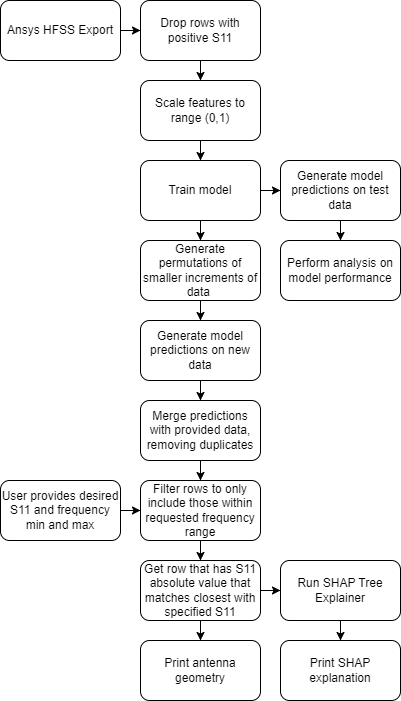
\includegraphics[width=3.0in]{methodology}
\captionof{figure}{Flow of data through the system}
\label{data_flow}
\end{Figure}

A GUI (graphical user interface) was created in order to make the process of filtering optimal geometries more intuitive. The GUI include an input area, where a user can input a desired $S_{11}$ and frequency range. Once these are entered, all of the permutations are filtered and the best performing optimal geometries are shown. A graph of frequency and predicted $S_{11}$ is also shown, where each optimal geometry is plotted. The desired $S_{11}$ and frequency range are also represented on the graph so it's clear what area of the graph is being focused on.


\section{Results}
\subsection{Library and Model Comparison with the Patch Antenna}
The patch antenna was used to test and compare the performance of models from the two different libraries: TensorFlow and Scikit-learn. The best performing model was chosen from each library, and their training time, predicting time, accuracy, and RMSE were compared in order to select the best model.

The Keras Tuner search for optimal hyperparameters of the DNN provided the results in Table~\ref{keras_best_params}. This was tested for both the patch antenna and the leaky wave antenna. The patch antenna was found to work best with a smaller DNN consisting of only two layers, where the leaky wave antenna performed best with more layers. The optimal learning rate was similar for both antennas, with the patch antenna having the higher learning rate. The DNNs were able to predict $S_{11}$ values with an error tolerance of~$\pm$1dB for the patch antenna and leaky wave antenna with a 84.17\% and 26.63\% accuracy respectively. These accuracies are not desirable, and might be an indicator that a DNN is too complex for this job.

\begin{table}[h]
\caption{Keras Tuner Best Hyperparameters}
\begin{center}
\begin{tabular}{ |l|l|l|l| }
    \hline
    Name & Patch Value & Leaky Wave Value \\ 
    \hline
    num\_layers & 2 & 3 \\  
    \hline
    units\_0 & 256 & 480 \\
    \hline
    units\_1 & 32 & 32 \\
    \hline
    units\_2 & N/A & 32 \\
    \hline
    learning\_rate & 0.0841 & 0.0250 \\
    \hline
\end{tabular}
\end{center}
\label{keras_best_params}
\end{table}

Figure~\ref{dnn_loss_graph} shows how the DNN's loss decreased as the number of epochs increased. The fact that this graph shows both the training and testing decreasing shows that the model is converging. Additionally, the model is not overfitting. 

\begin{Figure}
    \centering
    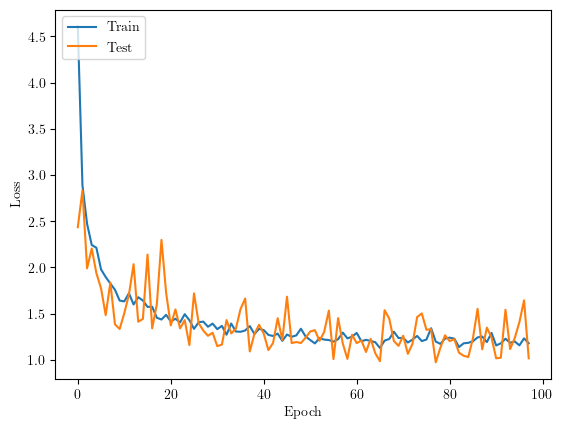
\includegraphics[width=2.5in]{loss}
    \captionof{figure}{DNN Loss Graph for Patch Antenna}
    \label{dnn_loss_graph}
\end{Figure}

Each of the Scikit-learn regression models performed differently than one another. After performing a randomized search for the best hyperparameters for each type of model, the score of the best configuration of each model was reported alongside the $R^2$ and RMSE scores. Please see Table~\ref{comparing_sklearn} for a summary of the results. The table is sorted by best to worst performance by score, RMSE, and $R^2$. The goal is to have the accuracy and $R^2$ closest to one, and the RMSE closest to zero. 

It's clear by looking at the table that RandomForestRegressor is the best performing model. It has the highest accuracy and the lowest RMSE, which proves that its predictions had the least distance from the actual $S_{11}$ values. When comparing TensorFlow to Scikit-learn, this is the model that will be used. 

\begin{table}[h]
\caption{Scikit-learn Results}
\begin{center}
\begin{tabular}{ |l|l|l|l| }
    \hline
    Model Type & Accuracy within~$\pm$1dB & RMSE & $R^2$ \\ 
    \hline
    RandomForestRegressor & 0.9301 & 0.7652 & 0.9620 \\
    \hline  
    DecisionTreeRegressor & 0.9080 & 1.0764 & 0.9248 \\  
    \hline
    GradientBoostingRegressor & 0.9012 & 0.9950 & 0.9357 \\
    \hline
    CatBoostRegressor & 0.8969 & 0.9949 & 0.9358 \\    
    \hline
    XGBRegressor & 0.8942 & 1.0467 & 0.9289 \\  
    \hline
    AdaBoostRegressor & 0.8526 & 1.1924 & 0.9077 \\  
    \hline
    SVR & 0.6717 & 2.7252 & 0.5180 \\  
    \hline
\end{tabular}
\end{center}
\label{comparing_sklearn}
\end{table}

When comparing the TensorFlow and Scikit-learn libraries, the same random state was used when splitting the data into training and testing portions. This ensures that each library is given a fair chance with the same set of data and the data isn't being swayed unintentionally. The TensorFlow model had 500 epochs, but only used 35 of them due to the early stopping criteria that was set. 

It's clear from the Table~\ref{comparing_libraries} that Scikit-learn is the best choice of library for this problem. The Scikit-learn model performed with 8.97\% better accuracy when predicting values with a tolerance of~$\pm$1dB. It trains and predicts significantly faster, and it has a lower RMSE.

\begin{table}[h]
\caption{Comparing Libraries}
\begin{center}
\begin{tabular}{ |l|l|l| }
    \hline
    Model Type & TensorFlow & Scikit-learn \\ 
    \hline
    Training Time (s) & 273.0s & 88.0 \\  
    \hline
    Predicting Time (s) & 2.91 & 3.69 \\
    \hline
    $S_{11}$ Accuracy within~$\pm$1dB & 0.8417 & 0.9314 \\
    \hline
    RMSE & 1.5050 & 0.7851 \\
    \hline
\end{tabular}
\end{center}
\label{comparing_libraries}
\end{table}

Figure~\ref{histogram_of_error_patch} shows how the Sklearn model had lower error between the predicted $S_{11}$ values and the actual $S_{11}$ values than the DNN model for the patch antenna. The DNN model tended to make predictions that were lower than the actual values. Additionally, Figure~\ref{actual_vs_predicted_s11_patch} demonstrates how the $S_{11}$ predictions were closer to the actual values, which is depicted by the diagonal line, for the Sklearn model. The DNN model had trouble predicting thet outliers. 

\begin{Figure}
    \centering
    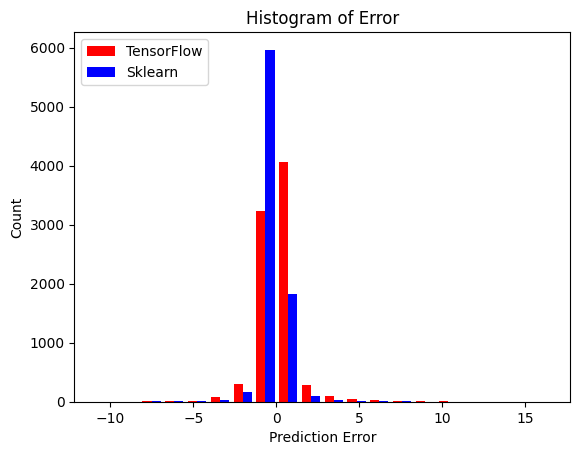
\includegraphics[width=2.5in]{histogram_patch}
    \captionof{figure}{Histogram of Error for Patch Antenna}
    \label{histogram_of_error_patch}
\end{Figure}

\begin{Figure}
    \centering
    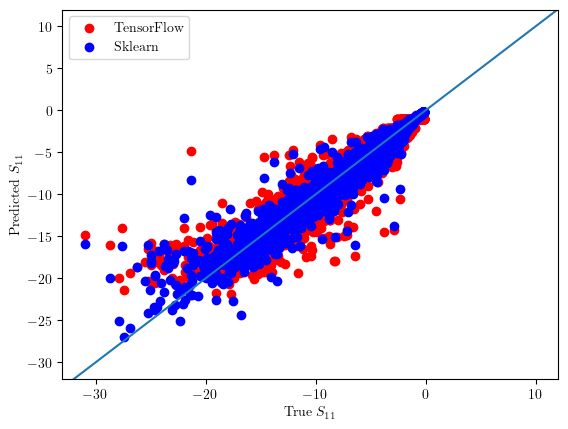
\includegraphics[width=2.5in]{actual_vs_predicted_s11_patch}
    \captionof{figure}{Actual vs Predicted $S_{11}$ for Patch Antenna}
    \label{actual_vs_predicted_s11_patch}
\end{Figure}

Figures~\ref{histogram_of_error_leaky_wave} and~\ref{actual_vs_predicted_s11_leaky_wave} show how the results for the leaky wave antenna are similar to those of the patch antenna. The leaky wave antenna was trained on significantly fewer geometries, which is reflected by the poorer overall performance of both the DNN model and the Scikit-learn model. Similarly to with the patch antenna, both figures prove that the Scikit-learn model makes $S_{11}$ predictions with higher accuracy than the DNN model.

\begin{Figure}
    \centering
    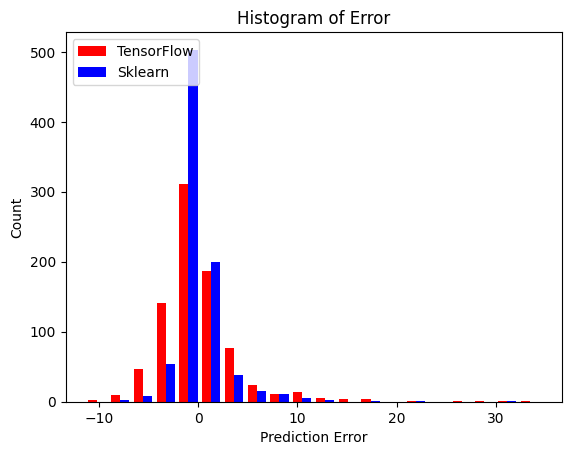
\includegraphics[width=2.5in]{histogram_leaky_wave}
    \captionof{figure}{Histogram of Error for Leaky Wave Antenna}
    \label{histogram_of_error_leaky_wave}
\end{Figure}

\begin{Figure}
    \centering
    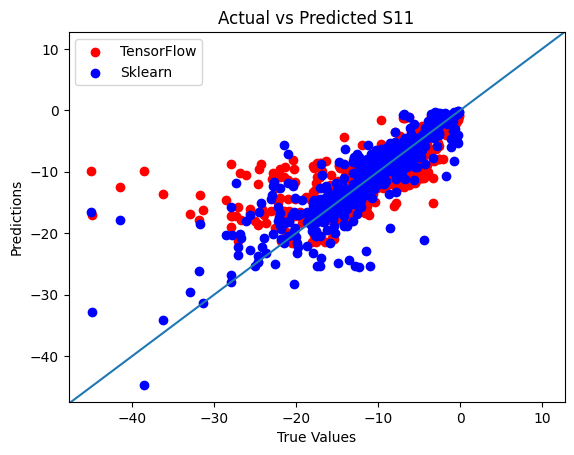
\includegraphics[width=2.5in]{actual_vs_predicted_s11_leaky_wave}
    \captionof{figure}{Actual vs Predicted $S_{11}$ for Leaky Wave Antenna}
    \label{actual_vs_predicted_s11_leaky_wave}
\end{Figure}

\subsection{Testing with Completely Unseen Geometries}
The chosen model was given a set of 6 random geometries from the patch antenna that had never been seen before by either the training set or testing set. These geometries were part of the permutations that were generated to create the dataset for optimal geometry searching. The geometric parameters of the chosen unseen geometries are recorded in Table~\ref{unseen_geometries}.

It's worth noting that each of the geometric parameters that were chosen for the unseen geometries lay within the range of the minimum and maximum value for each respective parameter. Due to the scaling that was performed during the preprocessing steps, any predictions made with geometric parameters that lay outside of the original range of the training data are capped as if the data point outside of the range was actually the corresponding minimum or maximum. Therefore, it didn't make sense to include any geometric parameters outside of the geometric parameters respective ranges. 

\begin{table}[h]
\caption{Unseen Geometry Parameters}
\begin{center}
\begin{tabular}{ |l|p{0.12\linewidth}|l|p{0.12\linewidth}|l|l|l| }
    \hline
    ID & inset\_dist [mm] & L [mm] & sub\_thick [mm] & W [mm] & W0 [mm] & y0 [mm] \\ 
    \hline
    1 & 0.6 & 11.5 & 2.0 & 14.8 & 2.5 & 4.25 \\
    \hline
    2 & 0.6 & 12.0 & 2.0 & 14.8 & 2.75 & 4.5 \\
    \hline
    3 & 1.0 & 12.0 & 2.0 & 15.6 & 3.5 & 4.25 \\
    \hline
    4 & 1.4 & 11.5 & 2.0 & 15.6 & 3.5 & 4.25 \\
    \hline
    5 & 1.4 & 11.5 & 2.0 & 15.4 & 3.5 & 4.5 \\
    \hline
    6 & 1.4 & 11.75 & 2.0 & 15.4 & 3.5 & 4.75 \\
    \hline
\end{tabular}
\end{center}
\label{unseen_geometries}
\end{table}

These unseen geometries were run through both the HFSS and the chosen machine learning model in order to obtain simulated and predicted $S_{11}$ values. This process was completed for the entire frequency range of the patch antenna. The results are shown in Figure~\ref{unseen_geometries_graph}, where each unseen geometry has its predicted $S_{11}$ values plotted alongside the simulated values for each frequency in the frequency range.

TODO WRITE more and actually update graph once cameron gets back to me 

\begin{Figure}
    \centering
    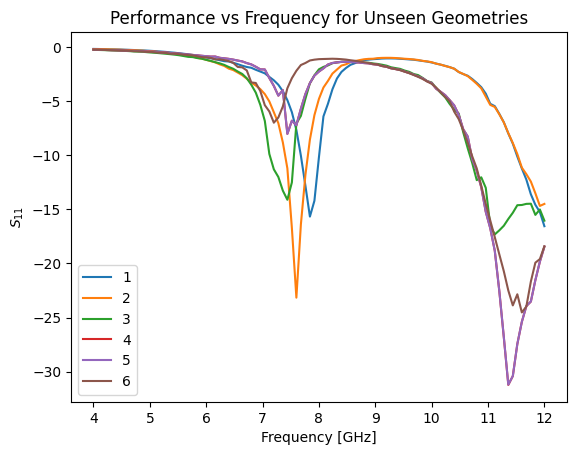
\includegraphics[width=2.5in]{unseen_geometries_freq_vs_seq}
    \captionof{figure}{Simulated \& Predicted $S_{11}$ Values for Frequency Range of Unseen Geometries}
    \label{unseen_geometries_graph}
\end{Figure}

\subsection{Finding Optimal Geometry}
TODO talk about gui here 

TODO replace image with something more high quality, find better example 

\begin{Figure}
    \centering
    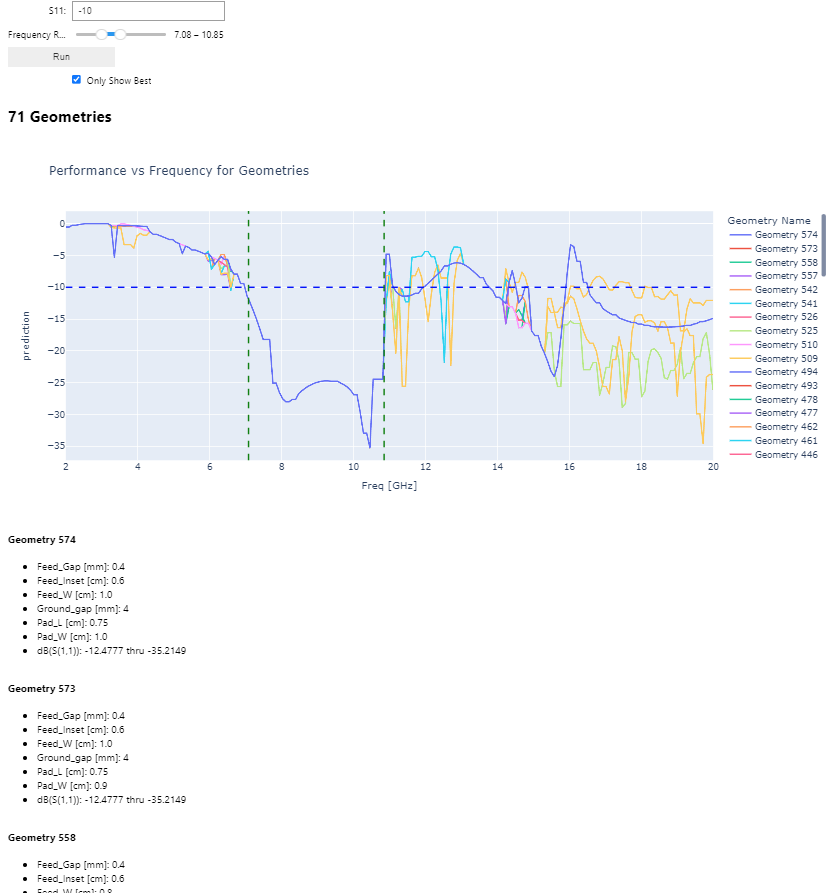
\includegraphics[width=2.5in]{gui}
    \captionof{figure}{Actual vs Predicted $S_{11}$}
    \label{gui}
\end{Figure}


\section{Conclusion}
Applying a machine learning algorithm as an aid in the process of optimizing  antenna geometric parameters with EM simulations greatly reduces the amount of time and computational power required. Training a model on a small set of data obtained from a parameteric sweep allows the model to fit to the trend of data. Large amounts of additional data can then be generated within the bounds of the existing data, and performance predictions can be made for this generated data with a high accuracy. The most optimal geometries can be returned for specified performance values and frequency ranges, making the trial-and-error process of finding these geometries by running simulations unnecessary. 

Using Scikit-learn regression models had better accuracy and lower training and testing times than a DNN built with TensorFlow. This is because the Scikit-learn models are simpler than a DNN and are more optimized for the task.  

TODO FINISH ME 


\section*{Acknowledgment}
The author would like to thank Cameron Martinez for his assistance in providing the datasets for both the patch antenna and the leaky wave antenna that were used for this research. Cameron was also very helpful in analyzing the performance of the models as compared to the actual simulated data. Additionally, the author would like to thank Dr.~Rojas and the WiDE Lab for providing support for this research and a space to work.


\bibliographystyle{IEEEtran}
\bibliography{refs}

\vfill

\end{document}